\documentclass[12pt]{article}
\usepackage[margin=1in]{geometry} 
\usepackage{amsmath}
\usepackage{amssymb}
\usepackage{siunitx}
\usepackage{float}
\usepackage{tikz}
\def\checkmark{\tikz\fill[scale=0.4](0,.35) -- (.25,0) -- (1,.7) -- (.25,.15) -- cycle;} 
\usepackage{url}
\usepackage[siunitx,american,RPvoltages]{circuitikz}
\ctikzset{capacitors/scale=0.7}
\ctikzset{diodes/scale=0.7}
\usepackage{tabularx}
\newcolumntype{C}{>{\centering\arraybackslash}X}
\renewcommand\tabularxcolumn[1]{m{#1}}% for vertical centering text in X column
\usepackage{tabu}
\usepackage[spanish,es-tabla,activeacute]{babel}
\usepackage{babelbib}
\usepackage{booktabs}
\usepackage{pgfplots}
\usepackage{hyperref}
\hypersetup{colorlinks = true,
            linkcolor = black,
            urlcolor  = blue,
            citecolor = blue,
            anchorcolor = blue}
\usepgfplotslibrary{units, fillbetween} 
\pgfplotsset{compat=1.16}
\usepackage{bm}
\usetikzlibrary{arrows, arrows.meta, shapes, 3d, perspective, positioning}
\renewcommand{\sin}{\sen} %change from sin to sen
\usepackage{bohr}
\setbohr{distribution-method = quantum,insert-missing = true}
\usepackage{elements}
\usepackage{verbatim}
\usetikzlibrary{mindmap,trees,backgrounds}
 
\definecolor{color_mate}{RGB}{255,255,128}
\definecolor{color_plas}{RGB}{255,128,255}
\definecolor{color_text}{RGB}{128,255,255}
\definecolor{color_petr}{RGB}{255,192,192}
\definecolor{color_made}{RGB}{192,255,192}
\definecolor{color_meta}{RGB}{192,192,255}
\usepackage[edges]{forest}
\usepackage{etoolbox}
\usepackage{schemata}
\newcommand\diagram[2]{\schema{\schemabox{#1}}{\schemabox{#2}}}
\usepackage{lastpage}
\usepackage{fancyhdr}
\usepackage{csvsimple,booktabs}
\pagestyle{fancy}
\setlength{\headheight}{42pt}
\usepackage{caption}
 
\begin{document}
\lhead{Ingeniería Física \\ Escuela de Física \\ Tecnológico de Costa Rica} 
\rhead{Instrumentación II \\ Tarea \#3  \\ Entrega: Semana 7} 
\cfoot{\thepage\ de \pageref{LastPage}}
\setlength{\parindent}{0em}

El satélite BATSU-CS1, enviado por el TEC y ACAE al espacio en 2018 era un satélite pequeño tipo CubeSat sin un sistema de control activo, cuando no existe control activo los paneles solares son iluminados de forma cambiante debido a la rotación del satélite, en \href{https://estudianteccr-my.sharepoint.com/:x:/g/personal/prof_juan_rojas_estudiantec_cr/ETTDDKfo78RMnVB7k3jrQuIBsd2N6uON5U7eSBfSzcLbxw?e=nt5Cpk}{este} archivo se puede descargar una simulación del comportamiento de la batería del satélite en una orbita completa (alrededor de 90 minutos). La baterías consiste de dos celdas de iones de litio tipo NCR18650B de Panasonic (Ver Figura \ref{fig:18650}). 

\begin{figure}[H]
    \centering
    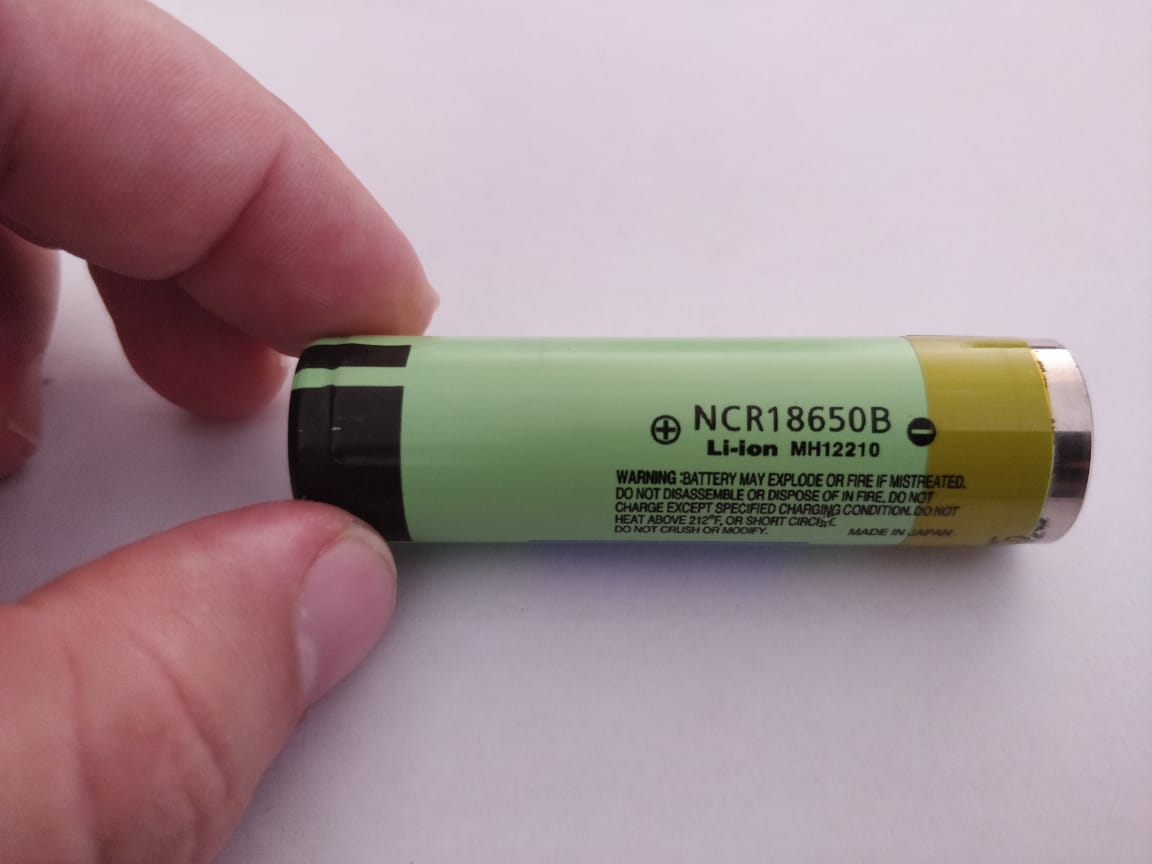
\includegraphics[width=0.6\linewidth]{fig/NCR18650.jpeg}
    \caption{Celda NCR18650B de Panasonic}
    \label{fig:18650}
\end{figure}

Algunos términos importantes sobre baterías:
\begin{itemize}
    \item Capacidad nominal [$Q$]: es la cantidad de carga que una celda o batería puede entregar en amperios-hora (\si{\ampere\hour}).
    \item Eficiencia de Coulumb [$\eta$]: es la eficiencia con la que se transfiere la carga a una batería, tipicamente se asume que $\eta = 1$ durante la descarga y que $\eta < 1$ durante la carga. 
    \item SOC [$z(t)$]: \emph{state of charge}, estado de carga de una celda o batería, para una celda o batería descargada $z(t) = 0$, mientras que para una celda o batería cargada $z(t) = 1$. El estado de carga se puede relacionar con la corriente por medio de la siguiente ecuación:
        \begin{equation*}
            z(t) = z(t_0) - \dfrac{1}{Q}\int_{t_0}^t \eta i(\tau) d\tau
        \end{equation*}
    La ecuación anterior se puede calcular a partir de datos discretos aproximando la integral que describe $z(t)$ por medio de una discretización con un intervalo $\Delta t$, esto es: 
        \begin{equation*}
            z[k+1] = z[k] - \dfrac{\eta \Delta t}{Q}i[k]
        \end{equation*}
    donde $\Delta t$ es el intervalo de integración discreta, en este caso $\SI{1}{\second}$; $z[k]$ e $i[k]$ son los valores actuales del SOC y la corriente respectivamente; y $z[k+1]$ es el valor siguiente del SOC
\end{itemize}

Algunos detalles importantes sobre la batería del CubeSat simulado:
\begin{itemize}
    \item La capacidad $Q$ es de \SI{6500}{\milli\ampere\hour}
    \item La eficiencia en descarga $\eta_d = 1$ y la eficiencia en carga es $\eta_d = 0.95$
    \item El estado de carga inicial $z(t_0)=0.4$ 
\end{itemize}

Algunos detalles importantes sobre las columnas del archivo:
\begin{itemize}
    \item La columna \emph{time} es el tiempo en segundos
    \item La columna \emph{current} es la corriente en amperios, cuando es negativa la batería se esta cargando, cuando es positiva la batería se esta descargando
    \item La columna \emph{voltage} es el voltaje en voltios
    \item La columna \emph{power} es la potencia en vatios
\end{itemize}

Usando LabVIEW desarrolle un instrumento virtual que realice lo siguiente:

\begin{itemize}
    \item Que lea el archivo facilitado usando una estructura adecuada, se recomienda el uso de indexación
    \item Que calcule el estado de carga $z(t)$ para todo tiempo en la columna \emph{time}
    \item Que detenga la ejecución de la estructura cuando se terminen los datos del archivo
    \item Que guarde todos los datos incluyendo la nueva columna \emph{soc} en un arreglo al terminar la ejecución
    \item Que guarde el arreglo generado en el archivo \verb+t3_out.csv+
    \item Guarde el instrumento virtual \verb+t3.vi+
    \item Incluya ambos archivos en un archivo comprimido \verb+t3.zip+ y subalo al TecDigital
\end{itemize}

Cualquier entrega tardía se califica en base a 70. 


% \bibliographystyle{IEEEtran}
% \bibliography{ref_tareas}

\end{document}